\documentclass[10pt,a4paper]{article}
\usepackage[utf8]{inputenc}
\usepackage[francais]{babel}
\usepackage[T1]{fontenc}
\usepackage{charter}
\usepackage[top=2cm, bottom=2cm, inner=2cm, outer=2cm]{geometry}
\usepackage{amsmath}
\usepackage{amsfonts}
\usepackage{amssymb}
\usepackage{graphicx}
\usepackage{lipsum}

\title{Figures avec \LaTeX \ \& Python}
\author{Aurélien Carré et Pierre Nagorny}
\begin{document}
\maketitle

\section{Hello}

\begin{figure}[h]
\begin{center}

\includegraphics[width = .5\textwidth]{fete-science.jpg}
\caption{Le logo de la fête de la science !}
\end{center}
\end{figure}

\section{Lorem ipsum dolor}

\lipsum[1-13]

\begin{figure}[h]
\begin{center}
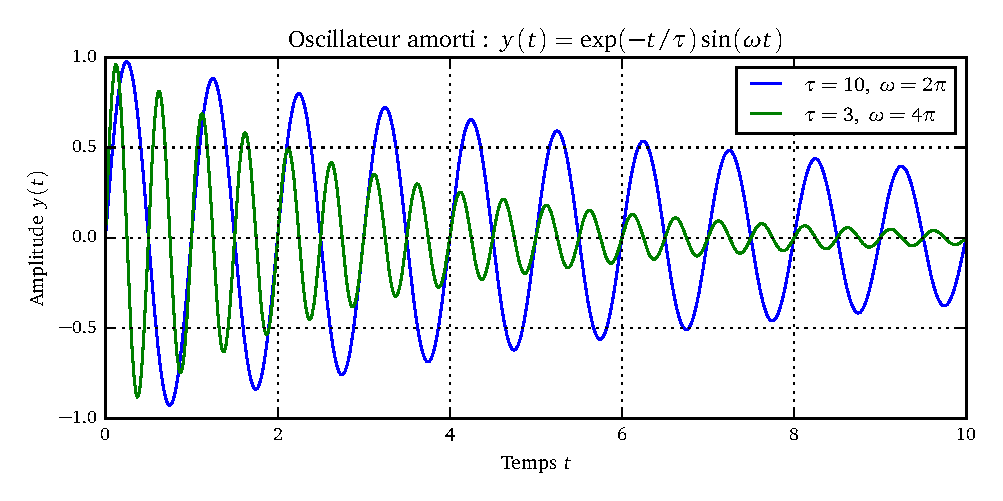
\includegraphics{Oscillateur}
\end{center}
\end{figure}

\lipsum[1-13]

\end{document}
